% Created 2017-08-19 Sat 09:30
\documentclass[11pt]{article}
\usepackage[utf8]{inputenc}
\usepackage[T1]{fontenc}
\usepackage{fixltx2e}
\usepackage{graphicx}
\usepackage{longtable}
\usepackage{float}
\usepackage{wrapfig}
\usepackage{rotating}
\usepackage[normalem]{ulem}
\usepackage{amsmath}
\usepackage{textcomp}
\usepackage{marvosym}
\usepackage{wasysym}
\usepackage{amssymb}
\usepackage{hyperref}
\tolerance=1000
\author{Anghelo De La Cruz}
\date{\today}
\title{ECON Unit 4}
\hypersetup{
  pdfkeywords={},
  pdfsubject={},
  pdfcreator={Emacs 25.2.1 (Org mode 8.2.10)}}
\begin{document}

\maketitle
\tableofcontents


\section{Nature and Operation of Budgetary Policy}
\label{sec-1}

\subsection{Definition}
\label{sec-1-1}

Budgetary policy (Also known as Fiscal Policy) refers to the
manipulation of the level and composition of Federal Government
receipts and outlays in order to assist in the achievement of its
economic and social goals for Australia. It is released annually each
May and contains estimates or projections of all income and
expenditure of the Government into the future. Though introduced in
May, new measures or 'mini budgets' can be taken by the Government.

\subsection{Objectives}
\label{sec-1-2}

The goal of all policies is to improve the welfare or living standards
of all Australians and to achieve the most efficient allocation of the
nation's resources.

This is achieved by:

\begin{itemize}
\item Strong and sustainable economic growth
\item Low inflation
\item Full Employment
\end{itemize}

This is clearly articulated in Government lesgilation (Charter of
Budget Honesty Act 1998)

\begin{quote}
The Government's fiscal policy is to be directed at maintaining the
on-going economic prosperity and welfare of the people of Australia
and is therefore to be set in a sustainable medium-term framework.
\end{quote}

\subsection{Composition of Revenue and Expenses}
\label{sec-1-3}

The Federal Government collects approximately \$411 billion per annum
in receipts from various sources.

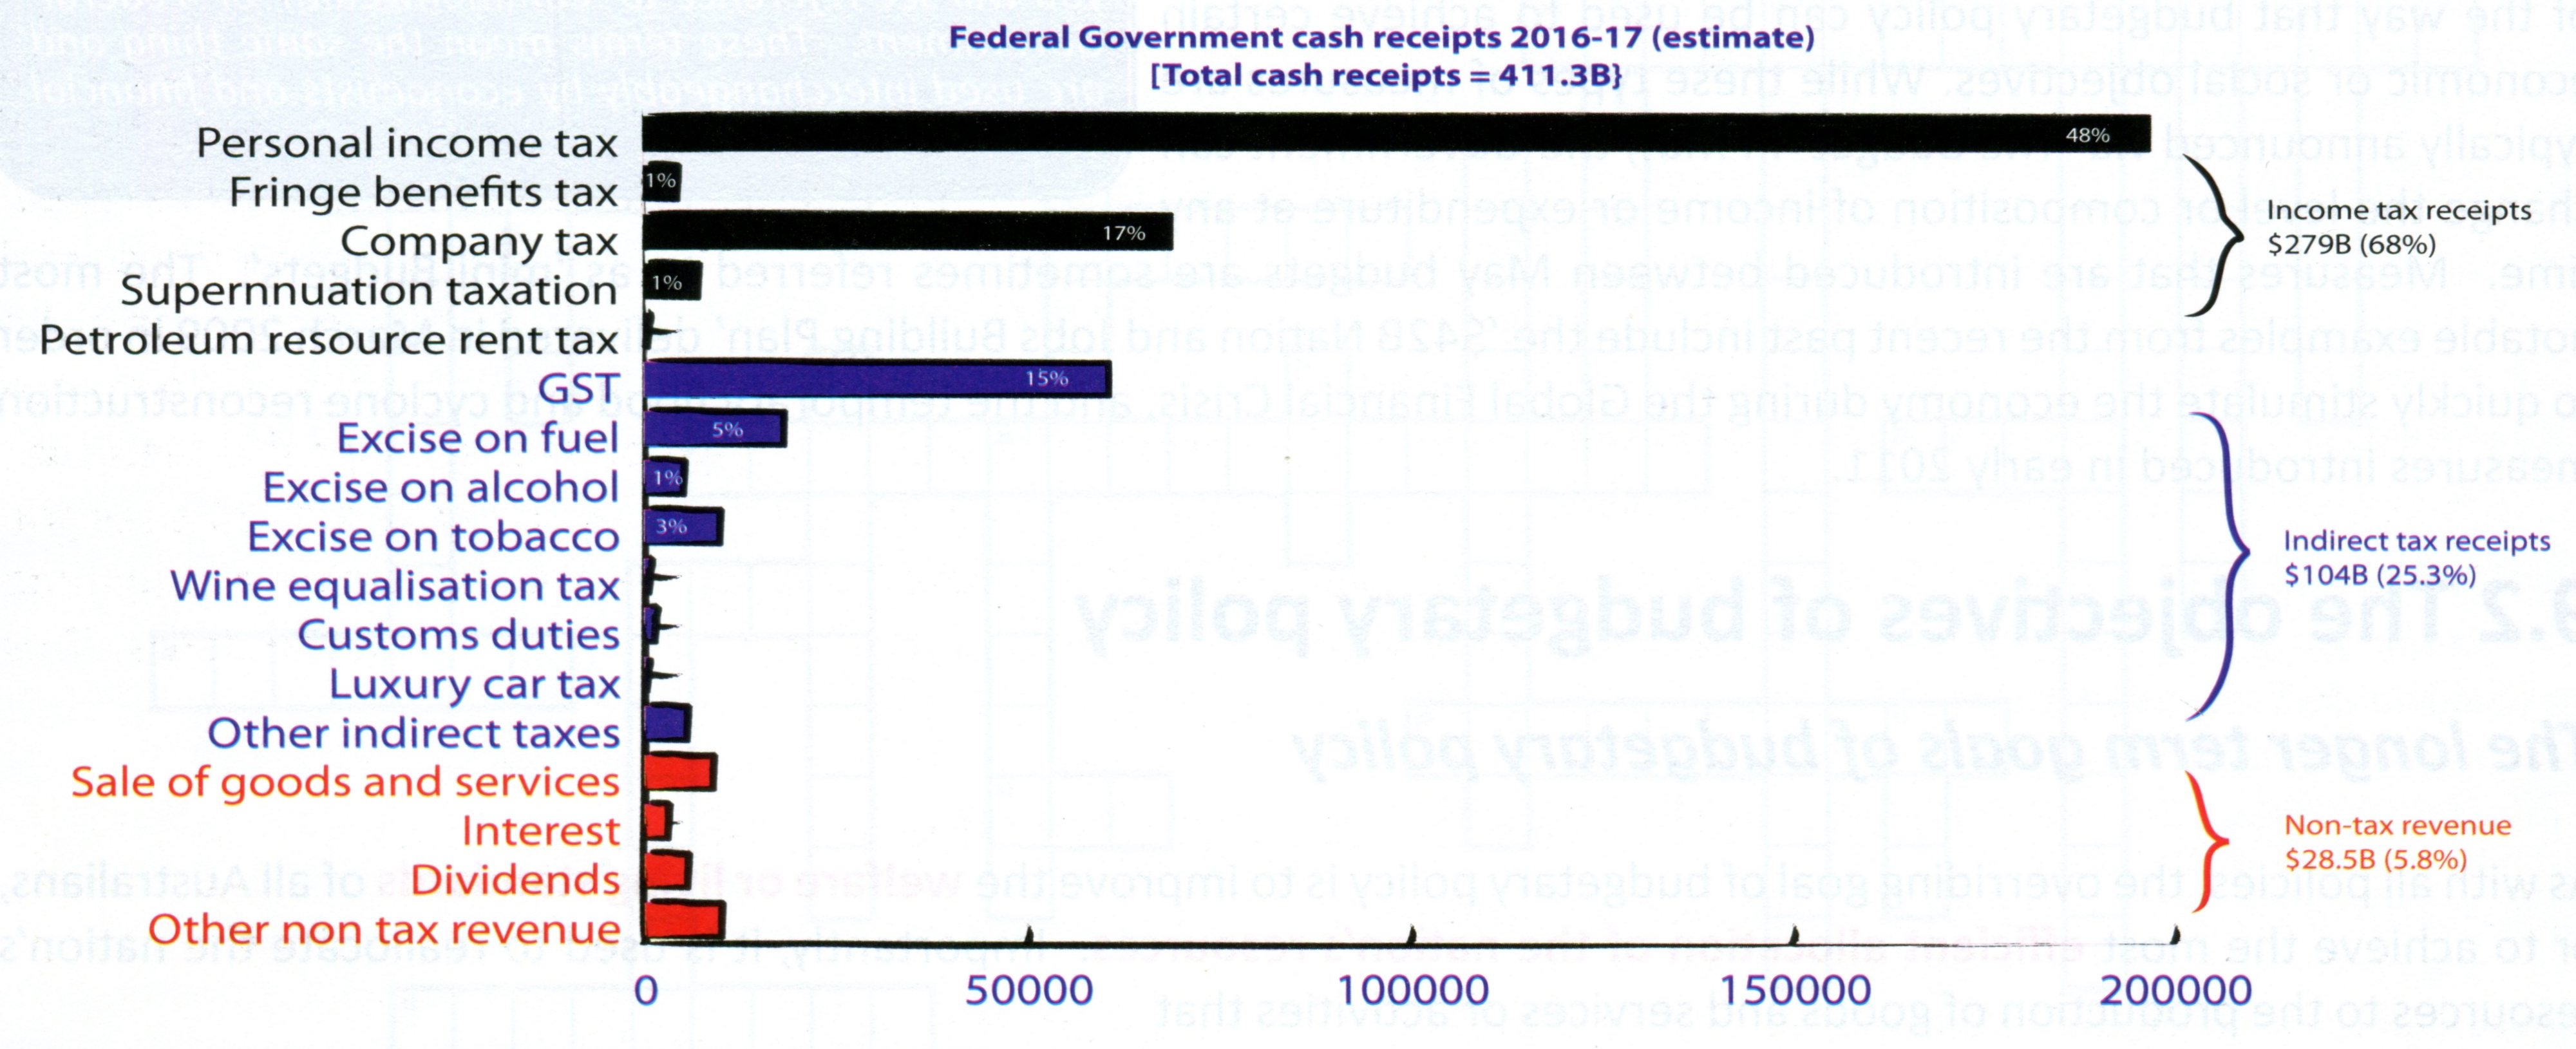
\includegraphics[width=.9\linewidth]{./images/Receipts.jpg}
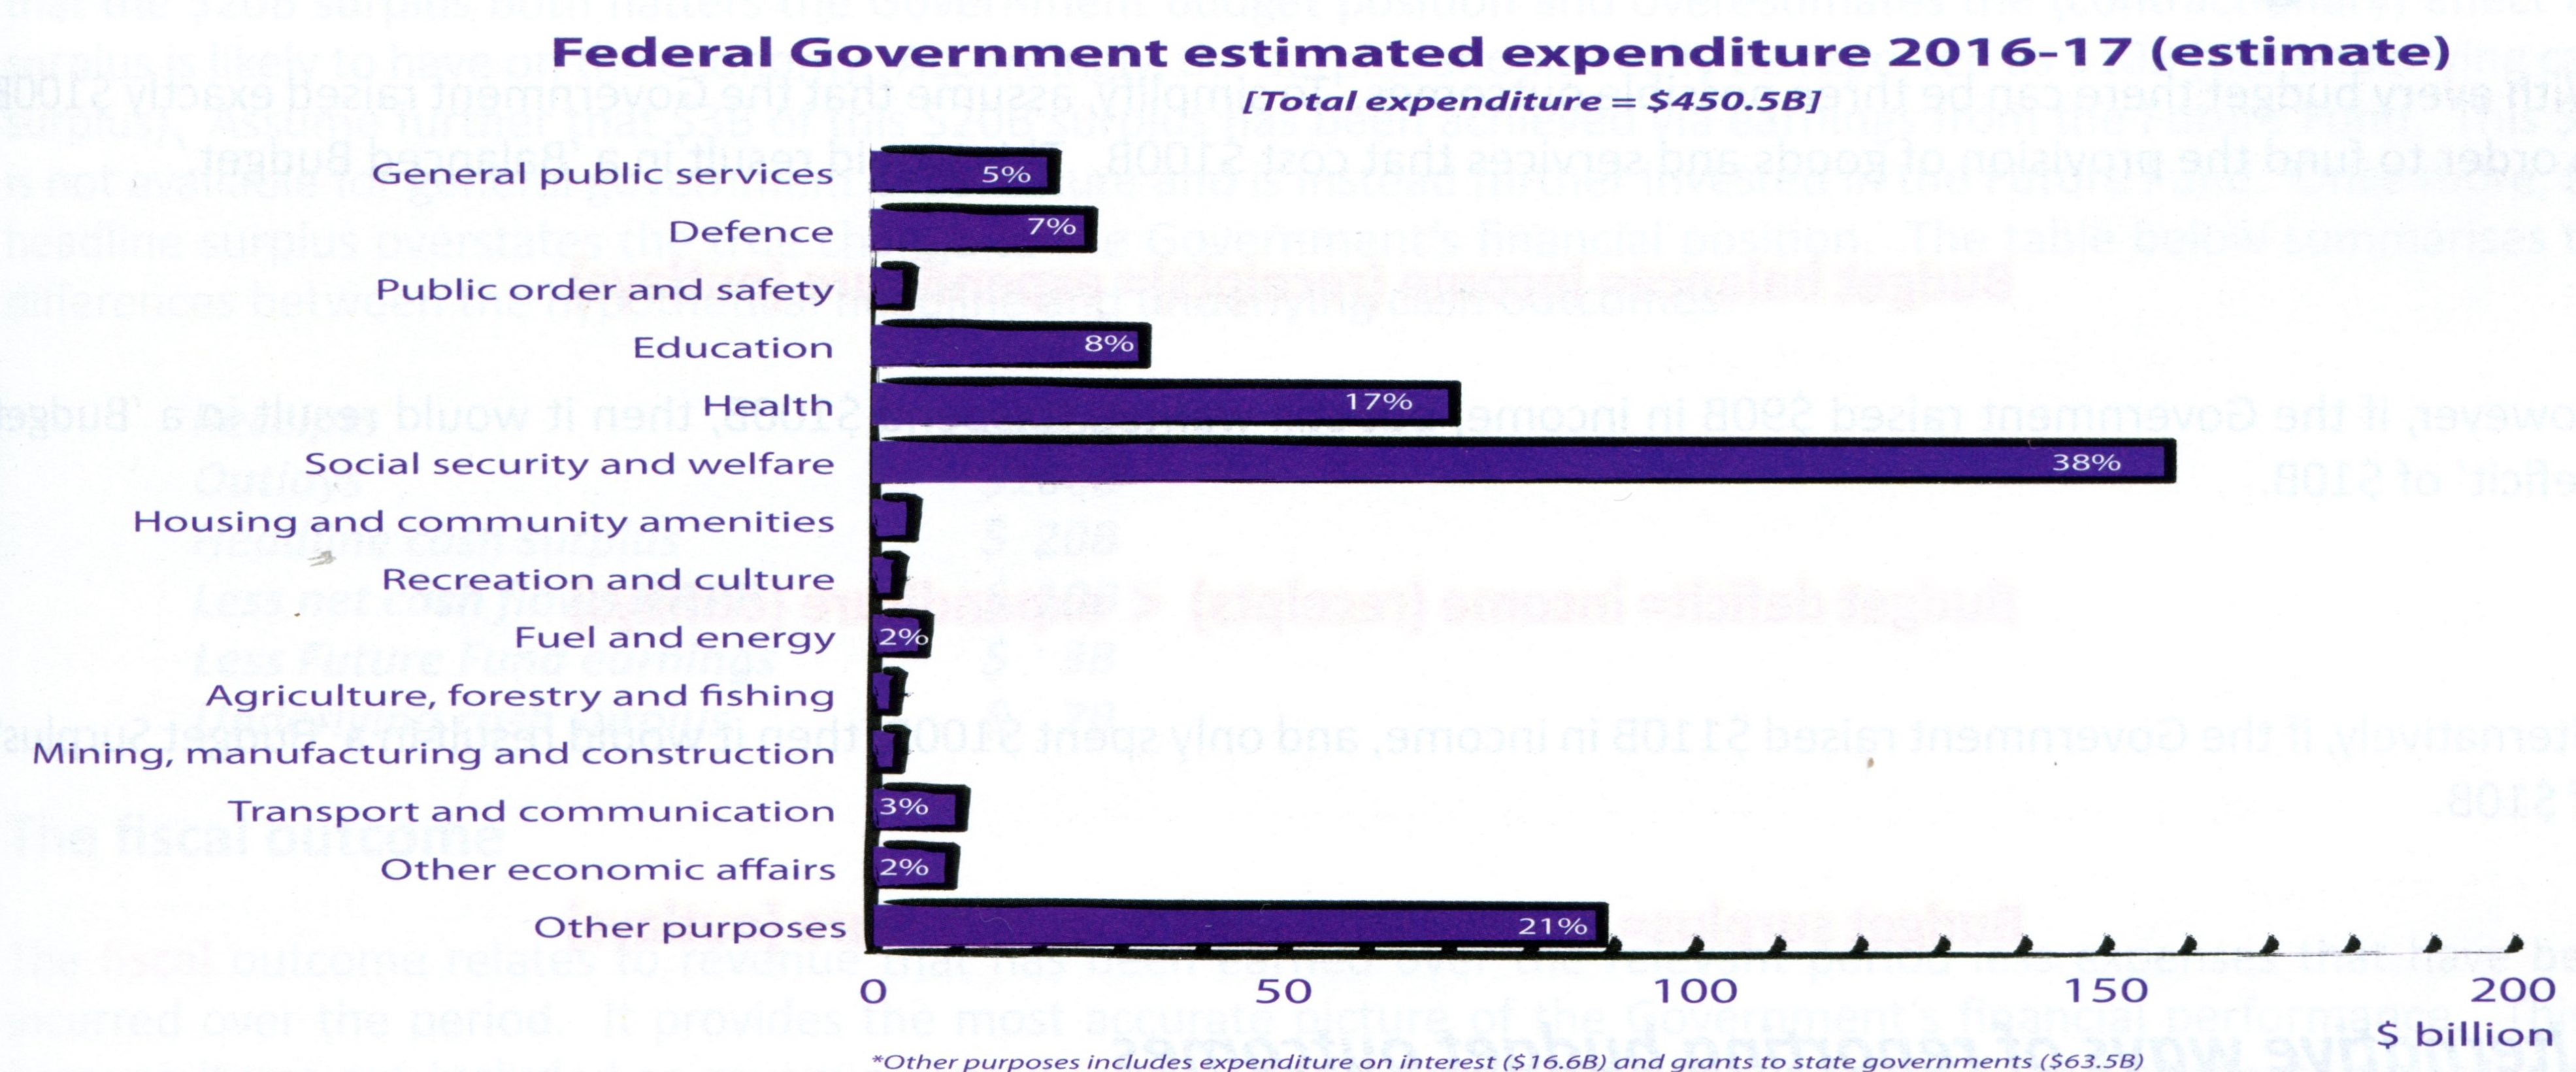
\includegraphics[width=.9\linewidth]{./images/Expenditure.jpg}


\subsection{Budget Outcomes}
\label{sec-1-4}

The Budget can have three possible outcomes:

\begin{align*}
        \text{Budget Balance} &= \text{Income(receipts)} = \text{Expenditure(outlays)}\\
    \text{Budget Deficit} &= \text{Income} < \text{Expenditure}\\
    \text{Budget Surplus} &= \text{Income} > \text{Expenditure}
\end{align*}

There are also several ways the Commonwealth Government will report
these outcomes.

\subsubsection{Headline Cash Outcome}
\label{sec-1-4-1}

This is the total cash received by the Federal Government subtracted
by the total cash paid. This can be misleading as it includes cash
flows that do not directly impact on the economy.

\subsubsection{Underlying Cash Outcome}
\label{sec-1-4-2}

This is the total cash received by the Federal Government subtracted
by the total cash paid. This can be misleading as it includes cash
flows that do not directly impact on the economy.

\begin{description}
\item[{Future Fund Earnings}] - interest and dividends earned by
government owned 'Future fund'. Excluded as earnings are mandated
to be reinvested.
\item[{IFAAP}] - Investments in financial assets for policy purposes;
including sale of government business enterprise (GBE),
purchases of shares by the government or granting or
repaying State Government debt. Excluded as does not
directly add to economic activity
\end{description}

To illustrate (using hypothetical figures):

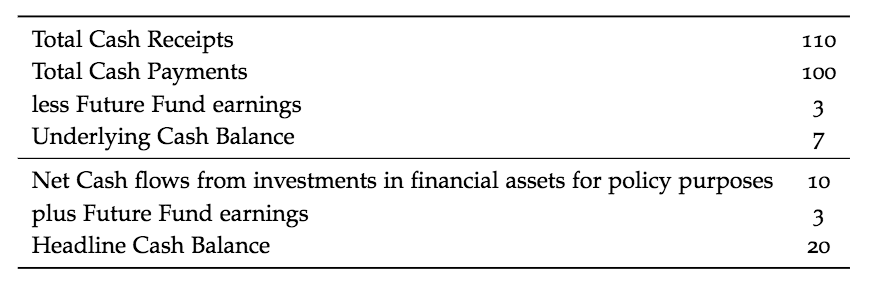
\includegraphics[width=.9\linewidth]{./images/Cash_Outcome.png}

\subsection{Automatic and Discretionary Stabilisers}
\label{sec-1-5}

Stabilisers - help to dampen the severity of booms and recessions in the business cycles.

2 types: 

\begin{description}
\item[{Discretionary}] fiscal / budgetary policy determined by the
government as per the annual budget
\item[{Automatic}] changes to the budget that occur automatically following changs in the level of economic activity
\end{description}

\subsubsection{Autmoatic}
\label{sec-1-5-1}

\begin{description}
\item[{Boom}] rising AD $\rightarrow$ higher employment, incomes and
profits
\begin{itemize}
\item Government tax revenues increases and welfare spending decreases
\item Fiscal system is automatically becoming contractionary
\end{itemize}
\item[{Recession}] falling AD $\rightarrow$ higher unemployment,
lower incomes and profits.
\begin{itemize}
\item Government tax revenues decreases and welfare payments increases
\item Fiscal situation is automatically becoming expansionary
\end{itemize}
\end{description}

Discretionary stabilisers are used when the automatic stabiliser are
not enough to correct a server boom or recession.




\subsection{Fiscal Drag / Bracket Creep}
\label{sec-1-6}

This occurs during times of inflation for countries with a progressive
tax system. When inflation occurs there is a decrease in the real wage
and workers will demand an increase in nominal wage to keep up with
inflatiion.

When the nominal wage increases, some workers are pushed into a higher
marginal tax bracket which increases the 'average' rate of tax paid.

These have two effects:

\begin{itemize}
\item Increases the total personal income tax revenue received by the
Federeal Government.
\item Some taxpayers will experience a decline in their real disposable
income because they will be paying a higher average rate of tax.
\end{itemize}


\subsection{{\bfseries\sffamily TODO} Actual and Estimated Budget Outcomes}
\label{sec-1-7}

The Department of Treasury releases the 'actual' budget figures for
the previous financial year in September or October (16 months after
the release of the budget).

\begin{description}
\item[{Estimated budget outcome}] released in May
\item[{Actual budget outcome}] released in September or October
\end{description}

The estimated budget outcome heavily relies on forecasts for economic
growth and other statistic which are never 100\% accurate.

\begin{center}
\begin{tabular}{ll}
Year 2 & \\
Receipts & \$100B\\
Outlays & \$120B\\
Headline cash deficit & \$20B\\
\end{tabular}
\end{center}






\subsection{{\bfseries\sffamily TODO} Expansionary v. Contractionary Budgets}
\label{sec-1-8}



\subsection{{\bfseries\sffamily TODO} Financing a Deficit / Investing a Surplus}
\label{sec-1-9}

\subsubsection{Budget Deficit $R < E$}
\label{sec-1-9-1}

Expansionary $\rightarrow$ Rise in AD which impacts on production,
employment and inflation

The gap is financed by government borrowing:

\begin{enumerate}
\item Borrow from public and financial sector by sale of bonds
\item Borrow from the RBA
\item Overseas borrowings
\end{enumerate}

\subsubsection{Budget Surplus $R > E$}
\label{sec-1-9-2}

Contractionary $\rightarrow$ Fall in AD

Use of surplus:

\begin{enumerate}
\item Save with RBA
\item Place in special investment or savings fund
\item Repay local and foreign debt
\end{enumerate}

\subsubsection{Problems with a expansionary budget deficit}
\label{sec-1-9-3}



\subsubsection{Dealing witha budget surplus}
\label{sec-1-9-4}

While a deficit tends to contribute to crowding out, a surplus tends
to do the opposite and contributes to crowding in of the private
sector.

\subsubsection{Fiscal consolidation and the rationale for delivering a budget surplus}
\label{sec-1-9-5}

\begin{itemize}
\item Help buffer Austraia against future economic decline as surplus
funds can be saved and then spent.
\item Helps to generate greater international investor confidence in
Australian government finances preserving Australia's AAA credit
rating.
\item Allows the cyclical component of the budget to do its job of
automatically reducing the deficit as the economy recovers.
\item Allows monetary policy to better manage the economy.
\end{itemize}

\subsection{{\bfseries\sffamily TODO} Budget and Economic Goals}
\label{sec-1-10}

In terms of Australia's specific domestic macroeconomic goals,
budgetary policy has a key role to play in the achieving of stability
in the level of domestic economic activity (also referred to as
\textbf{Internal Stability})

\subsubsection{Stablising the business cycle}
\label{sec-1-10-1}

\subsubsection{Changing role of Budgetary Policy}
\label{sec-1-10-2}

\subsubsection{Budgetary policy and low inflation}
\label{sec-1-10-3}

\subsubsection{Budgetary policy and strong and sustainable growth}
\label{sec-1-10-4}

\subsubsection{Budgetary policy and ull employment}
\label{sec-1-10-5}

\subsection{{\bfseries\sffamily TODO} Budgetary Policy and Living Standards}
\label{sec-1-11}

\subsection{Strengths and weaknesses of Budgetary Policy}
\label{sec-1-12}
\subsubsection{Strengths}
\label{sec-1-12-1}
\begin{itemize}
\item Target particular sectors
\item Greater range of economic goals
\item Impact lag
\item Effictively stimulating AD
\item Effect through automatic stabilisers
\item Checks and balances
\end{itemize}
\subsubsection{Weakness}
\label{sec-1-12-2}
\begin{itemize}
\item Political hurdles
\item Political bias
\item Imlementation lag
\item Inflexible
\item Less effective at restricting AD during a boom
\end{itemize}



\section{Budgetary policy in Action}
\label{sec-2}

\subsection{Recent use of the budget}
\label{sec-2-1}

\subsection{Evaluating the effectiveness of budgetary policy}
\label{sec-2-2}

\subsection{Specific budgetary policy initiatives}
\label{sec-2-3}


\subsection{Budget Examples}
\label{sec-2-4}

\subsubsection{Growth}
\label{sec-2-4-1}

\subsubsection{Unemployement}
\label{sec-2-4-2}

\begin{enumerate}
\item Youth Employment Packages
\label{sec-2-4-2-1}

\item Skilling Australians Fund
\label{sec-2-4-2-2}
\end{enumerate}

\subsubsection{Inflation}
\label{sec-2-4-3}

\section{{\bfseries\sffamily TODO} Monetary Policy}
\label{sec-3}

Relies on changing the level of interest rates to alter the cost,
demand and availability of credit. It has fast impact and does not
require the involvement of parliament.

\subsection{Role of RBA:}
\label{sec-3-1}

\begin{itemize}
\item banker to the government, banks, and NBFIs (Non-bank Financial
Institute)
\item Issues notes and coins
\item custodian of overseas currency reserves
\end{itemize}

\textbf{Priority} is low inflation; as it is a precondition to achieving
 consumer and business confidence.

RBA board meets monthly on Tuesday (except January), and considers the
following economic data:

\begin{itemize}
\item Quarterly trends in headline CPI
\item Spending levels (C), (I)
\begin{itemize}
\item Building approvals
\item Household debt
\end{itemize}
\item Unemployment rate
\begin{itemize}
\item Job vaccancies
\item Participation
\end{itemize}
\item Overseas markets
\item Government budgetary stance.
\end{itemize}

Monetary Policy works in a counter cylical pattern.

\subsection{Definition}
\label{sec-3-2}

Monetary policy is operated by the RBA on behalf of the government and
involves the manipulation of key financial variables in the economy
(primarily interest rates) in order to achieve specific economic goals
and ultimately improve the living standards or welfare of all
Australians. The medium term objective is 'stability of the
currency', which the RBA currently defines as price stability, where
consumer price inflation is kept between 2 and 3 per cent, on average,
over time.

The RBA will only be concerned if inflation is outside the range for a
'sustained' period. Once low inflation is achieved, the RBA can then
focus on policy decisions that assist in the attainment.

\subsection{Objectives}
\label{sec-3-3}

\begin{itemize}
\item the stability of the currency of Australia
\item the maintenance of full employment in Australia
\item the economic prosperity and welfare of the people of the Australia.
\end{itemize}

Monetary policy will generally be useed in a counter-cyclical way to
boost activity when inflation and growth are low and restrain activity
when inflation and growth are high.

\subsubsection{Underlying rate of Inflation}
\label{sec-3-3-1}



\subsubsection{Financial Stability}
\label{sec-3-3-2}



\subsection{Implementation}
\label{sec-3-4}

\subsection{Cash rate and Open Market Operations}
\label{sec-3-5}

The RBA manipulates the cash rate by buying and selling \textbf{Commonwealth
Government Securities (CGS)} or repurchase agreements (repos) to
participants in the cash market (primarily banks). This manipulation
of the cash market is commonly referred to as \textbf{open market operations
(OMOs)} or domestic market operations.

\subsubsection{Diagram 11.1 Pg 310}
\label{sec-3-5-1}

\subsubsection{Target Cash Rate}
\label{sec-3-5-2}

\subsection{Monetary Policy Tightening / Loosening}
\label{sec-3-6}



\subsection{Monetary Policy Settings}
\label{sec-3-7}

\subsection{Tranmission Mechanism}
\label{sec-3-8}

\subsubsection{Cost of Credit Channel (Savings and Investment)}
\label{sec-3-8-1}

\subsubsection{Cash Flow Channel}
\label{sec-3-8-2}

\subsubsection{Availability of Money / Credit Channel}
\label{sec-3-8-3}

\subsubsection{Asset Values / Asset Price Channel}
\label{sec-3-8-4}

\subsubsection{Exchange Rate Channel}
\label{sec-3-8-5}

\subsection{Exchange rate intervention}
\label{sec-3-9}



\subsection{Strengths and weeknesses of Monetary Policy}
\label{sec-3-10}

\subsubsection{Strengths}
\label{sec-3-10-1}

\begin{itemize}
\item Free from political bias
\item Short Implementation lag
\item Powerful influence on consumers, investors, borrowers or lenders
\item Good at restraining AD as policy reduces discretionary income of
indebted households.
\end{itemize}

\subsubsection{Weaknesses}
\label{sec-3-10-2}

\begin{itemize}
\item Is one dimensional and unable to concentrate its affect on a speicific area
\item Full impact can take up to two years (Impact lag)
\item RBA does not have direct control over interest rates. This could
mean financial insitutions won't pass on 'in full' the reductions in
the cash rate.
\item A reduction in interest rates may not immediately increase AD
because consumers are not forced to spend any increase in
discretionary income.
\item Policy becomes less effectve as levels of private sector
indebtedness increase to high levels.
\item Policy cannot directly reduce inflationary pressures that are
generated from the supply side of the economy (cost inflation). This
will instead only ignite demand inflationary pressures, worsening
inflation overall.
\end{itemize}


\section{{\bfseries\sffamily TODO} Monetary Policy in Action}
\label{sec-4}

\subsection{Price Stability}
\label{sec-4-1}

\subsection{Stronger Economic Growth and Employment}
\label{sec-4-2}

\subsection{Stabilisation of the Business Cycle}
\label{sec-4-3}

\subsection{Living Standards}
\label{sec-4-4}

\subsection{Specific Policy Changes Over the Cycle}
\label{sec-4-5}

\begin{center}
\begin{tabular}{llll}
Year & Policy Stance & Monetary Policy & Context\\
Late 2007 &  &  & Economic Growth relatively high. Economy capacity constraints.\\
Early 2008 & Restrictive &  & Inflaion 5\%\\
Mid 2008 &  &  & GFC\\
2009 &  &  & Target rate falling to 'emergency levels' of 3\%\\
November 2010 &  &  & RBA concerned about the emergence of capacity constraints and the implications for inflation\\
2011 & Restrictive &  & \\
2011-2012 & Loosened & Reduced target cash rate back to 3\% by December by 2012 & \\
2013 & Loosened & Target cash rate 2.5\% by August 2013 & \\
2014 &  & Target cash rate remained at 2.5\% through 2014 & 'Persistance' with expansionary stance\\
2015 &  &  & Falling TOT, RBA felt stimulus was required\\
Late 2015 &  &  & Economy performing relatively poorly, economic growth below trend, Unemployment at 6.3\% August 2015\\
 &  &  & \\
\end{tabular}
\end{center}
% Emacs 25.2.1 (Org mode 8.2.10)
\end{document}
